\begin{center}
    \textbf{--------- Lezione 3 - 6 ottobre 2020 ---------}
\end{center}

\section{Le reti cellulari}
Le reti cellulari permettono ad un dispositivo mobile di trasmettere voce e dati attraverso un'infrastruttura distribuita nel territorio composta da:
\begin{itemize}
    \item Antenne: sono sparse nel territorio ed ognuna di queste ha una copertura limitata. Per permettere ai dispositivi di avere una copertura sufficiente (una copertura geografica), ci sono molte antenne
    \item Varie componenti di elaborazione delle informazioni 
\end{itemize}

Nascono negli anni ’80 e si sono rapidamente evolute. Esempi di tecnologie: GSM, GPRS, EDGE, LTE.
\\ Queste tecnologie sono organizzate in generazioni (es. 1G, 2G, 3G, ecc.) dove ogni generazione stabilisce delle performance di riferimento. 
Le diverse tecnologie condividono una stessa architettura.

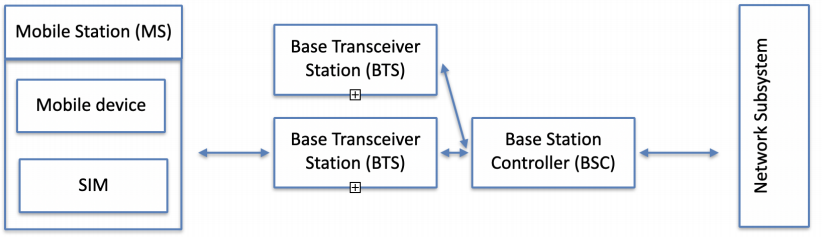
\includegraphics[width=\textwidth]{images/Mobile computing/3. Reti e architetture/architettura.PNG}

La \textit{SIM} è una componente HW che ha la scopo di identificare e autenticare l'utente per l'accesso alla rete. 
Le \textit{Mobile Station (MS)} includono due componenti: la SIM e il device.
La SIM contribuisce a funzioni di sicurezza in quanto contiene chiavi crittografiche utilizzate per realizzare la comunicazione di rete. 
\\ La mobile station comunica via radio con una componente chiamata \textit{Base Transceiver Station (BTS)} che include una o più antenne per la comunicazione e un hw di gestione dell'informazione per gestire il segnale in ingresso e in uscita. Ogni BTS è collegata al \textit{Base Station Controller (BSC)} che coordina varie BTS e a sua volta comunica con l'infrastruttura di rete chiamata \textit{Network Subsystem}. 

La potenza del segnale diminuisce all'aumentare della distanza tra la MS e l’antenna.
La distanza massima di comunicazione dipende dal tipo di tecnologia.
ma in linea di massima entro la quale si può comunicare è anche di diversi chilometri. 
Per erogare il servizio su una scala geografica, sono sparse nel territorio le BTS. 
Ciascuna BTS definisce una cella, cioè una regione geografica dove il segnale di quella BTS è più forte, rispetto al segnale delle BTS circostanti. 
Man mano che ci allontaniamo dall'antenna entriamo in un'altra cella perché il segnale di quest'altra antenna è più forte della precedente. 

Ogni BTS comunica con varie MS tramite onde radio, su intervalli di frequenze che sono specificati dal protocollo utilizzato.
Ogni intervallo è suddiviso in un numero finito di portanti che sono a loro volta suddivise in uplink e downlink (comunicazione verso la BTS).
Ad esempio GSM ha 248 portanti nell'intervallo attorno ai 900MHz.
\\ Ogni portante è suddivisa in canali usando tecniche di FDM (frequency division multiplexing) e TDM (time division multiplexing).
\\ Ogni MS nel momento in cui comunica con la BTS necessita di un canale in uplink e uno in downlink. Il numero massimo di MS che possono comunicare con una stessa BTS è limitato. 
In zone ad alta densità di popolazione è necessario avere celle più piccole, per suddividere la popolazione tra più BTS.
In questo caso una procedura, chiamata session handover, permette il passaggio di controllo di una mobile station ad un'altra e il dispositivo non si accorge di essere passato da un'antenna all'altra. L'IP del telefono rimane invariato. 

\section{Le architetture per dispositivi mobili}
Molto spesso le applicazioni di dispositivi mobili fanno parte di un sistema distribuito e comunicano con un server ed altri dispositivi mobili. 

Ci sono fattori che influenzano molto la progettazione della app:
\begin{itemize}
    \item la connessione potrebbe andare persa. Nei dispositivi mobili è anche normale che l'accesso ad Internet avvenga tramite diversi tipi di connessione che cambiano nel tempo
    \item il tipo di connessione cambia. In alcuni casi grazie al session handover è possibile mantenere la stessa connessione anche quando un dispositivo si sposta all'interno di una rete cellulare, ma la stessa funzionalità non è disponibile quando un dispositivo si sposta tra reti diverse e dunque riceve un nuovo indirizzo IP. Ad esempio un utente è connesso alla rete WiFi di casa, quando esce si connette alla rete cellulare e quando arriva a lavoro si connette ad un'altra rete WiFi che gli assegnerà un nuovo IP
\end{itemize}

\subsection{Connection-oriented vs connection-less}
I due fattori portano a sconsigliare l'utilizzo di protocolli connection-oriented dove si ha una connessione prolungata tra le due entità che comunicano.
Non è consigliabile perché il dispositivo perde la connessione e siccome ho una connessione aperta tra client server, se il client cambia l'indirizzo IP, la connessione va persa.

Nei protocolli connection-less invece non viene mantenuta una connessione prolungata tra due componenti. 
Queste comunicazioni sono più adatte ai dispositivi mobili. 

In un'architettura client-server, il server espone delle API (chiamate) che i client possono sfruttare per portare a termine il loro compito. 

\subsection{Architettura three-tier}
Lo schema architetturale three-tier è comunemente utilizzato per erogare servizi web. 
Il browser fa una richiesta HTTP al web server che legge e scrive i dati su un DB. Una volta che il web server termina la scrittura e la lettura dei dati, esegue lo script lato server, recupera il file necessario ed esegue il codice PHP che può richiedere di interagire con una base di dati. Il web server al browser ritorna la pagina html, il codice javascript che esegue lato client e dei css.
\\ PHP è lo scripting lato server e non viene eseguito lato client, javascript invece è lo scripting lato client e non viene eseguito lato server.

L'architettura per i dispositivi mobili è molto simile.
L'applicazione comunica con un web service tramite HTTP. Il web spesso comunica con un DB che memorizza l'informazione in modo persistente. 
Una delle differenza principali è che l'applicazione client
solitamente riceve dal web service solo i dati richiesti, in quanto il comportamento dell'applicazione, incluse le informazioni su come formattare i dati ricevuti, fanno già parte dell'applicazione stessa. I dati possono essere scambiati in un qualunque formato, incluso il testo semplice. Tuttavia, per dati complessi esistono vari formati, tra cui XML e JSON.

\begin{figure}
    \centering
    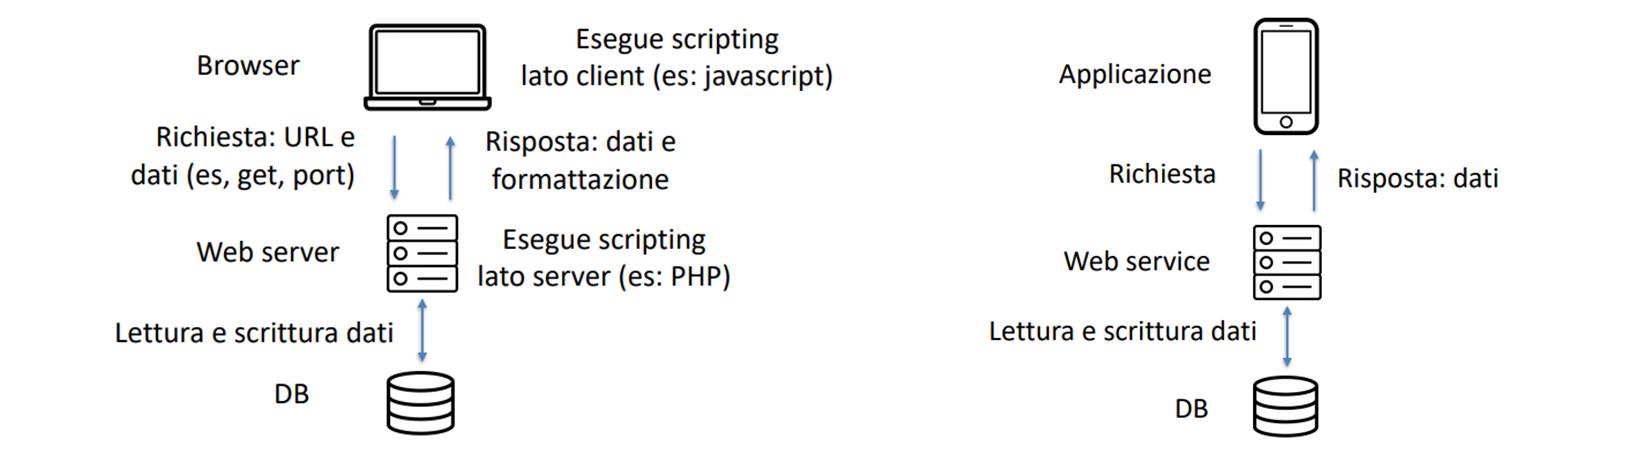
\includegraphics[width=\textwidth]{images/Mobile computing/3. Reti e architetture/architettura tt.png}
    \caption{Schema del modello three-tier applicato al web (sinistra) e alle applicazioni (destra)}
    \label{fig:architettura tt}
\end{figure}

I modelli presentano due componenti diversi:
\begin{itemize}
    \item web server: un server che fornisce informazioni (generalmente HTML+CSS+JS) finalizzate ad essere mostrate (tramite un browser) all'utente 
    \item web service: un server fornisce informazioni finalizzate ad essere ricevute da un’applicazione (anche mobile)
\end{itemize}

Quando facciamo un sistema vero, vogliamo far si che un sistema sia utilizzabile sia su app che su web e vorremmo evitare di scrivere due volte il codice.
Quello che si fa è usare un web server che manda tutti i contenuti al browser e che gli permettono di avere lo stesso comportamento dell'app mobile. 
\\ Invece di avere web service e web server, abbiamo un web service che interagisce con l'applicazione e poi il web server che passa semplicemente al browser la web app. 

\begin{figure}[!ht]
    \centering
    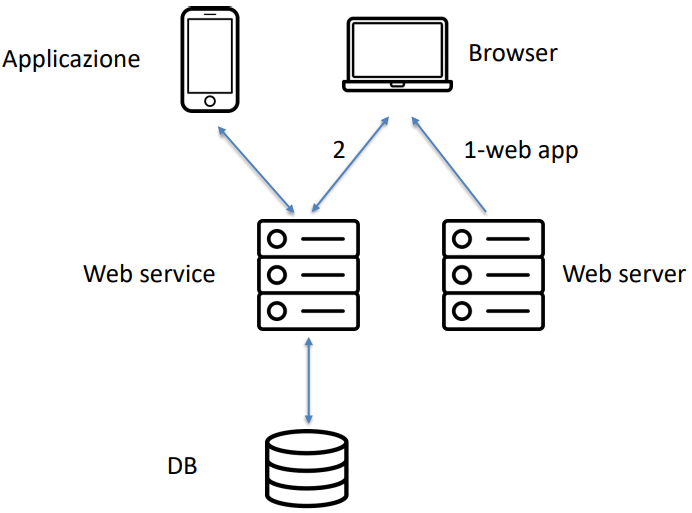
\includegraphics[width=.5\textwidth]{images/Mobile computing/3. Reti e architetture/app_web.PNG}
    \caption{Architettura per supportare contemporaneamente l'accesso da browser e da applicazioni}
    \label{fig:sistemi web_app}
\end{figure}

\subsection{La definizione del protocollo di comunicazione}
Progettare un protocollo di comunicazione non è facile. Vogliamo definire API sul server con le quali i client possono interagire: scambiare i dati con il server e ottimizzare il volume di dati scambiati, tenendo conto dei vincoli dei dispositivi mobili e permettendo una buona esperienza utente. 

Il protocollo è di tipo connection-less. Le chiamate avvengono con connessioni diverse, ma solitamente sono logicamente legate le une alle altre. Bisogna definire in quale ordine avvengono, in quali situazioni, quali dati si devono scambiare, ecc.

\subsubsection{Esempio di comunicazione}
Pensiamo ad un social. Ogni utente ha un profilo (con nome e foto) e uno stato (online o offline). Vogliamo che un utente possa scaricare la lista degli amici. 
\\ Il modo più semplice per implementare questa cosa è richiedere al server l'elenco dei contatti. 
È una soluzione semplice, ma ogni volta che l'utente vuole accedere alla lista, deve riscaricare tutti i contatti (con la foto, il nome e lo stato). 

Un'altra soluzione sarebbe di andare a scaricare in locale gli amici, in modo tale che una seconda volta scarico solamente quelli che precedentemente non avevo ancora scaricato (ad esempio un nuovo amico).
Qui ho un altro problema, perché se un amico aggiorna la foto profilo, io in locale ho quella vecchia. 

La soluzione corretta e ottimizzata è quella di utilizzare un contatore. Per ogni utente il server gestisce un contatore delle foto di profilo caricate (un numero di versione). Quando un utente scarica l’elenco degli amici il server gli manda, per ciascuno, il numero di versione della foto (è un dato di dimensione irrilevante rispetto ad un’immagine). Per ogni amico verifico se ho già salvato in locale la foto giusta e nel caso la mostro, altrimenti chiedo la foto al server e poi la salvo in locale per la prossima volta.

\begin{figure}[!ht]
\begin{center}
    \subfloat[Aggiornamento delle foto]{\fbox{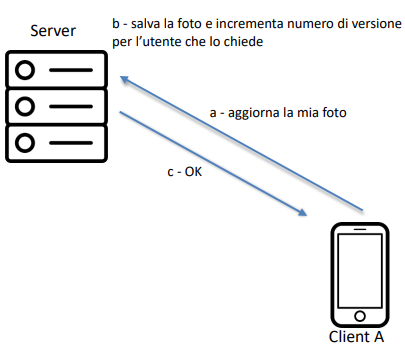
\includegraphics[width=.4\textwidth]{images/Mobile computing/3. Reti e architetture/1.PNG}}}
    \qquad \subfloat[Scarico lista amici]{\fbox{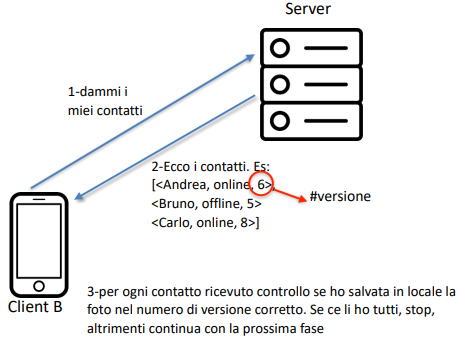
\includegraphics[width=.45\textwidth]{images/Mobile computing/3. Reti e architetture/2.PNG}}}
    
    \subfloat[Scarico foto aggiornate]{\fbox{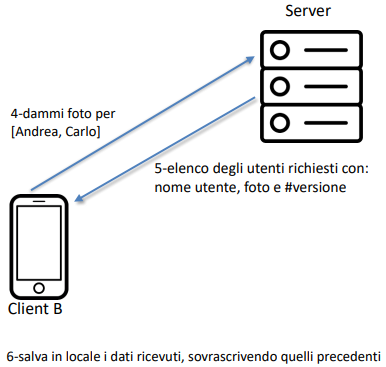
\includegraphics[width=.4\textwidth]{images/Mobile computing/3. Reti e architetture/3.PNG}}}   
\end{center}
\caption{Trasmissione delle immagini profilo in un social network}
\label{fig:immagini social}
\end{figure}
\newpage

\section{La codifica dell'informazione}
In una richiesta HTTP è possibile trasmettere informazioni in testo semplice. 

Prendiamo ad esempio un servizio che prende una parola in input e risponde con un sinonimo.
L'output è sempre una stringa e se non viene trovata nessuna corrispondenza, ritorna la stringa vuota.

Prendiamo ad esempio, invece, un servizio che data una parola in input risponde con una lista sinonimi. 
In questo caso potremmo ad esempio usare una codifica di parole separate da virgole. 

Diventa peggiore se data una parola in input, risponde con una lista di sinonimi e una di contrari.
Dobbiamo rappresentare due liste di parole e potemmo inventarci un modo per separare le due liste, per esempio usare il punto e virgola per separare.

Esistono degli strumenti che ci permettono di codificare l'informazione come ad esempio XML e JSON.

XML è un linguaggio di markup che permette di definire formati dei dati che sono “human and machine readable”. 

Un documento XML è ben formattato se rispetta alcune regole (ad esempio se tutti i tag sono aperti e poi chiusi). 
XML presenta alcuni limiti:
\begin{itemize}
    \item tende ad essere verboso 
    \item non facilmente leggibile da umani
    \item gli schemi XML sono abbastanza difficili da definire e spesso vengono ignorati
\end{itemize}

Un esempio di risposta XML per il servizio dictionary:
\begin{XML}
    <dictionary entry="nice">
        <synonyms>
            <word>pleasant</word>
            <word>agreeable</word>
            <word>enjoyable</word>
        </synonyms>
        <antonyms>
            <word>ugly</word>
            <word>unpleasant</word>
        </antonyms>
    </dictionary>
\end{XML}

JSON concettualmente svolge lo stesso lavoro di XML, cerca di ridurre la verbosità e di migliorare la lettura. 
\\ Un esempio di risposta JSON per il servizio dictionary:
\begin{JSON}
    {
        "entry":"nice",
        "synonyms ":[" pleasant","agreeable","enjoyable"],
        "antonyms ":[" ugly","unpleasant"]
    }
\end{JSON}    

XML definisce delle entità, JSON definisce degli oggetti. 
Sono due rappresentazioni diverse, ma concettualmente sono analoghi, infatti rappresentano i dati di un elemento che vogliamo descrivere.

Un'entità in XML o un oggetto JSON mi definisce uno stato nel mondo reale ma non il comportamento, nei linguaggi di programmazione invece un oggetto definisce sia lo stato che il comportamento ad esso associato. 
Questa distinzione è molto importante in quanto esiste una forte correlazione tra le strutture dati dei programmi e la codifica in XML o JSON. 

\subsection{Serializzazione e deserializzazione}
In memoria principale lavoriamo con oggetti dei linguaggi di programmazione ma questi oggetti non possono transitare in rete. Quello che ci serve è andare a convertirli nella propria rappresentazione XML o JSON. Questa operazione si chiama \textit{serializzazione} (o \textit{marshalling}). Il risultato è una stringa (internamente codificata in XML o JSON). L'entità che riceve la comunicazione di rete può leggere questa stringa e
riconvertirla in struttura dati tramite un’operazione che si chiama \textit{deserializzazione} o \textit{unmarshalling}.
Uno dei vantaggi nell'uso di XML o JSON è che le operazioni di serializzazione e deserializzazione sono supportate, in quasi tutti i linguaggi di programmazione, da apposite librerie.
Un esempio di queste librerie è GSON. 
\\ GSON è lo strumento di conversione, JSON è il formato di rappresentazione.

\subsection{Codifica di dati binari}
Sia in XML che in JSON vengono rappresentati i dati singoli nella loro codifica testuale. Non c'è nessun problema per stringhe, interi, float, boolean, ecc, ma si pone un problema per i dati binari ad esempio le immagini.
Il modo più comune è la codifica Base64 che permette di rimappare la codifica binaria dell'informazione in alcune informazioni testuali.
\\ Definisco una conversione tra 64 simboli (caratteri ASCII) e un valore numerico: A=1, B=2, ecc.
Scelgo dei caratteri ASCII che non mi introducano confusione nelle rappresentazioni XML o JSON (es: non uso "$<$", né ",").
Un simbolo rappresenta dunque 6 bit ($2^6$ = 64).
Dunque per rappresentare 3 byte in binario mi servono 4 simboli (3*8 = 4*6).
Per convertire da binario a Base64 suddivido l’input in gruppi di 3 byte, codifico ciascun gruppo con 4 simboli Base64.
Si usa la Base64 perché è una codifica testuale che usa meno caratteri per rappresentare e perché permette di non utilizzare caratteri strani. 

\subsection{Protocol Buffer}
Protocol Buffer è il protocollo definito da Google per serializzare le informazioni. Risolve lo stesso problema di XML e JSON definendo non solo il formato di scambio, ma anche gli strumenti SW di (de)serializzazione.
\\ Protocol Buffer è un protocollo:
\begin{itemize}
    \item multi-piattaforma, multi-linguaggio 
    \item ottimizzato in termini di dimensione del messaggio da scambiare 
    \item che risolve diversi problemi tipici ad esempio la gestione della versione dei protocolli 
\end{itemize}
\vspace{2em}